\section{Product Perspective}
\label{sec:product_Perspective}

\subsection{Scenarios}
\label{subsec:scenarios}

\newcounter{scenario}
\setcounter{scenario}{1}
\newcommand{\incscenario} {\stepcounter{scenario}}

\begin{itemize}
    \item \textbf{\nth{\thescenario} Scenario: Sign Up and Profile Creation Performed by a Student}
    \\
        Marco Stella, a student at Politecnico di Milano, wants to find a suitable summer internship to put into practice the knowledge gained during his Bachelor's Degree in Computer Science. 
        He has discovered the opportunity offered by the S\&C platform and has decided to sign up in order to browse the advertised internships. He is required to provide the necessary information in order to subscribe, such as his educational email, password, and other personal details. Once the account verification process has been completed, Marco is asked to upload his CV and potentially add other relevant details about his background, skills and attitudes.
        Once this information is inserted into the platform, all the functionalities provided by S\&C get enabled and he can freely navigate his personal dashboard, finally able to start the search process.
        \incscenario
    \item \textbf{\nth{\thescenario} Scenario: Sign Up and Profile Creation Performed by a Company}
    \\
        BrightFuture, a company specializing in AI solutions, is looking to recruit talented interns to support its upcoming projects. The company has heard about the opportunities provided by the S\&C platform and decides to register in order to post internship offers and connect with potential candidates.
        To begin, a representative from BrightFuture Technologies signs up by providing the necessary company details, such as the corporate email address, password, and additional contact information about the organization. Once the account registration is complete, the system sends a confirmation email for verification. After confirming the email, the representative is prompted to create a company profile: this involves adding essential details, such as a description of the organization, its mission, and the fields it operates in. They can also upload the company logo and other branding elements to enhance the profile’s appeal to prospective interns.
        With the profile fully set up, BrightFuture Technologies can now access all the features of the S\&C platform, including its personalized dashboard.
        \incscenario
    \item \textbf{\nth{\thescenario} Scenario: Publication of an Internship Offer by a Company}
    \\
        TechFuture, a company specializing in the development of innovative software solutions, decides to use the S\&C platform to post an internship opportunity for students interested in the tech industry. After logging into their corporate account using their credentials, a representative selects the "Create New Offer" option from the main menu.
        The platform prompts the company to provide all the necessary details for the internship: the application domain, the tasks to be performed, the required skills, the duration of the internship, the application deadline and the compensation terms. The representative carefully completes all the required fields, reviews the information for accuracy, and submits the offer.
        The system performs an automatic preliminary verification of the provided details to ensure the offer complies with the platform’s policies and standards. Once the review is completed, the internship offer is published on the platform, making it accessible to students who can now apply and explore the opportunity further.
        \incscenario
    \item \textbf{\nth{\thescenario} Scenario: Internship Search by a Student}
    \\
        Davide Bianchi, a second-year Mechanical Engineering student at Politecnico di Milano, is eager to find an internship that aligns with his academic background and career aspirations. He logs into the S\&C platform using his credentials and navigates to the "Search Offers" section.
        Here, the platform presents him with a search interface, allowing him to apply filters to narrow down the opportunities based on his preferences. Davide specifies his criteria: internships related to mechanical design, located in Italy, with a duration of at least three months. Confident in his choices, he submits the search.
        Within moments, the system displays a list of internship offers that match Davide's selected criteria. Browsing through the options, he identifies a position posted by Innovex Solutions, a company known for its innovative mechanical systems.
        The platform confirms that the student has been successfully added to the offer's applicants list. Encouraged by this seamless process, he continues exploring other opportunities to further expand his options.
        \incscenario
    \item \textbf{\nth{\thescenario} Scenario: Automatic Internship Recommendation}
    \\
        Luca Rossi, a second-year Electrical Engineering student at Politecnico di Milano, has recently completed his profile on the S\&C platform. His profile includes details about his academic background, skills, and interests, which he hopes will help him find an ideal internship opportunity.
        As part of its functionality, the S\&C platform automatically analyzes Luca’s profile. It leverages the information he has provided - such as his field of study, technical skills, and career aspirations - to compare it with the internship offers available on the platform. Using a recommendation algorithm, the system identifies the internships that best align with Luca’s qualifications and professional goals.
        Once the analysis is complete, the platform compiles a list of recommended internships. Luca receives a notification informing him about the new recommendations. He navigates to the "Recommendation" section, where he can review the suggested opportunities and start applying for positions that match his interests and attitudes.

        \incscenario
    \item \textbf{\nth{\thescenario} Scenario: Automatic Student Recommendation}
    \\
        GreenSpark Energy, a company specializing in renewable energy solutions, has recently posted an internship offer on the S\&C platform. The offer outlines the required skills, academic background, and other criteria for the ideal candidate. Once the offer is published, the platform's recommendation system begins its analysis.
        The system retrieves the details of the internship, such as the field of study, necessary qualifications, required skills, and desired attributes. Using these parameters, it compares the offer against the profiles of students registered on the platform. Leveraging its recommendation algorithm, the system identifies a list of students whose profiles closely align with the internship requirements.
        Once the analysis is complete, the platform compiles a list of recommended candidates. The system notifies GreenSpark Energy and provides access to the list of students, allowing the company to review their profiles and directly invite them to apply for the internship. 
        \incscenario
    \item \textbf{\nth{\thescenario} Scenario: Managing an Interview between a Company and a Student}
    \\
        Innovex Solutions, a company specializing in innovative mechanical systems, is reviewing applications for a recently posted internship position. Among the candidates, they identify Davide Bianchi, a promising Mechanical Engineering student at Politecnico di Milano, whose profile aligns closely with their requirements. The company decides to invite him for an interview.
        Through the S\&C platform, Innovex Solutions sends an interview invitation to Davide, including the date, time, and format (video call or in-person). Shortly after, Davide receives a notification about the interview and logs into the platform to review the details. Finding the schedule convenient, he accepts the invitation and confirms his availability.
        On the agreed date, the interview is conducted as planned. During the session, Davide discusses his qualifications, skills, and aspirations, while the company representative provides more information about the role and evaluates his suitability.
        After the interview, Innovex Solutions uses the platform to post the results of the interview, informing Davide whether he has progressed to the next stage of the selection process or been offered the internship.
        The system updates Davide's status in the selection process, ensuring he remains informed about the outcome. 
        \incscenario
        
    \item \textbf{\nth{\thescenario} Scenario: Reporting and Handling Problems during an Internship}
    \\
        Giulia Moretti, a Civil Engineering student at the Politecnico di Milano, is excited to begin her internship at Skyline, a company specializing in urban infrastructure projects. On her first day, Giulia is welcomed by her supervisor, who outlines her responsibilities and assigns her to work on a sustainability-focused bridge design project. The initial weeks of her internship are productive, with Giulia learning new skills and gaining hands-on experience.
        Throughout the internship, Giulia and her supervisor at Skyline regularly update the S\&C platform with progress details. Giulia logs her completed tasks, acquired skills, and challenges faced. These updates help both the university and Skyline monitor the alignment between Giulia’s work and her learning objectives.
        However, midway through the internship, Giulia encounters a significant issue: the tools and resources promised by Skyline for her project, including access to specific engineering software, are unavailable. This lack of resources makes it difficult for Giulia to complete her assigned tasks effectively. After attempting to resolve the issue internally with her supervisor without success, Giulia decides to report the problem to her university.
        Using the S\&C platform, Giulia navigates to the "Report Problems" section and submits a detailed description of the issue. She explains the nature of the problem, its impact on her project, and the steps she has already taken to address it. The platform immediately makes Giulia's report available to her university’s internship coordinator.
        Upon receiving the report, the university’s coordinator reviews the details and contacts both Giulia and Skyline to discuss the issue. During a scheduled meeting, the coordinator gathers additional information from both parties and assesses the situation. After evaluating the options, the university decides to address the issue by coordinating with Skyline to speed up the software licensing process. The problem is resolved within a week, and Giulia is able to continue her internship with minimal disruptions.
        As the internship progresses, Giulia continues to log her tasks and achievements on the S\&C platform. Finally, the internship reaches its scheduled conclusion. Giulia submits final feedback summarizing her work, the skills she has developed, and her overall experience. Skyline also provides formal feedback through the platform, highlighting Giulia’s strengths and suggesting areas for further improvement.
        Both the student's and the company’s feedback is stored in the system and fed to the recommendation mechanisms, allowing the evaluation of the quality of internships offered by Skyline and the improvement of future recommendations. 
        \incscenario
    \item \textbf{\nth{\thescenario} Scenario: Profile Optimization Suggestions for Students}
    \\
        Alessandro Romano, a second-year Computer Science student at Politecnico di Milano, logs into the S\&C platform to ensure his profile is fully optimized for attracting internship opportunities. Navigating to his profile page, he notices a notification prompting him to review suggestions for improvement.
        The system automatically analyzes Alessandro’s profile, considering his academic background, skills, and documents such as his CV. Based on the analysis, the platform generates a list of personalized suggestions. These include adding programming languages that are in high demand, updating his project portfolio, and providing a more detailed description of his certifications.
        Alessandro reviews the suggestions carefully and starts implementing the changes directly through the platform.
        \incscenario
    \item \textbf{\nth{\thescenario} Scenario: Internship Offers Optimization Suggestions for Companies}
    \\
        BlueHorizon Robotics, a company specializing in autonomous systems and AI integration, logs into the S\&C platform to ensure its internship offers are effectively attracting top candidates for their internship programs. A representative navigates to the page of one of their offers and notices a prompt indicating available optimization suggestions.
        The platform’s system analyzes the offer and the company's profile details, including details about past internship postings, descriptions of ongoing projects, and the clarity of their technical requirements. Based on the analysis, the platform generates actionable suggestions, such as refining the job description to better outline the scope of responsibilities or specifying advanced technical skills required for certain roles.
        The representative carefully reviews the suggestions and begins updating the offer's description to align with the recommendations.
        \incscenario
\end{itemize}

\subsection{Domain-level Class Diagram}
\label{subsec:domain_level_class_diagrams}

\begin{figure}[H]
    \begin{center}
        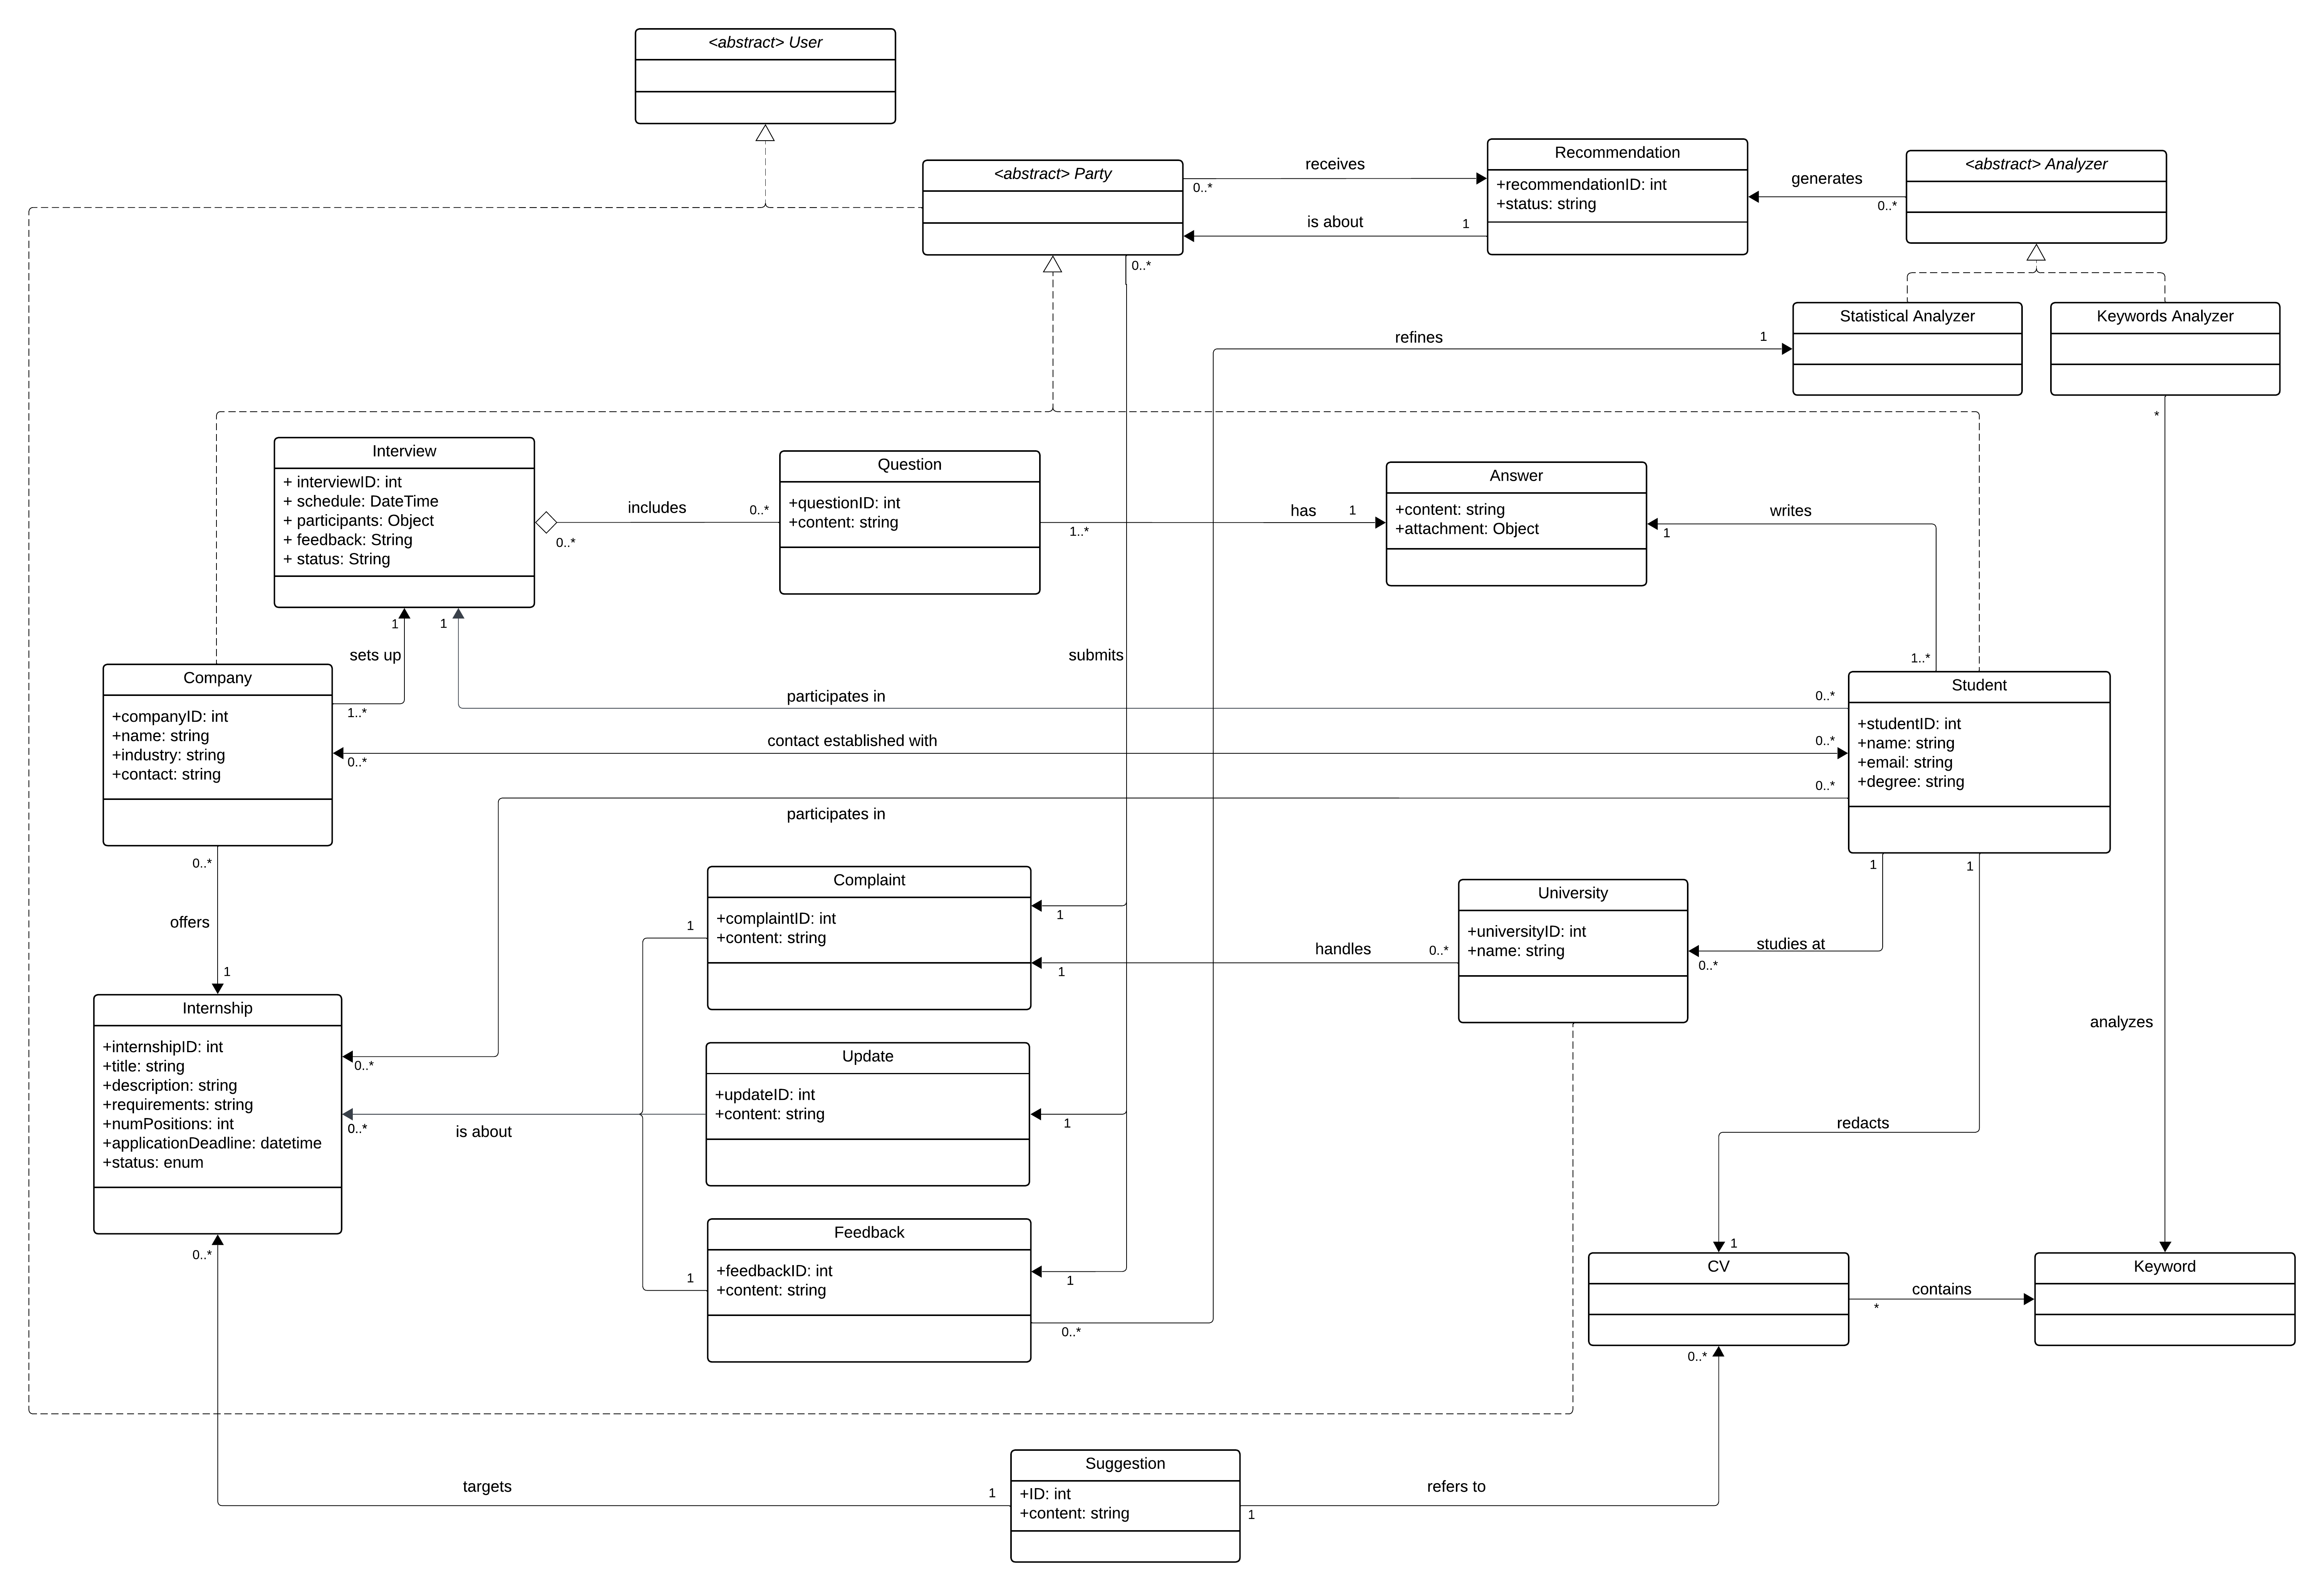
\includegraphics[width=0.9\linewidth]{LaTeXCode/images/Class Diagram - RASD.png}
        \caption{Domain-Level Class Diagram.}
        \label{fig:domain_level_class_diagrams}
    \end{center}
\end{figure}

The entities interacting with the system are modeled through a hierarchical structure to aggregate common functionalities. At the top level, the User class generalizes all the users of the system. From it, the University and Party classes derive, with the latter further specialized into the Student and Company entities.

The core of the system revolves around the concept of connecting students with internship opportunities: this is reflected in the relationships between the Student, Company, and Internship entities. The Student entity encapsulates candidate data such as personal details and educational background, which combined with the CV class, are essential to matching students with adequate internship opportunities. Companies can publish detailed internship offers that students can eventually search and apply for.

The Recommendation entity serves as a link between CVs and Internships, enabling the system to suggest the most relevant opportunities to students and identify suitable candidates for companies. This process is asymmetric, as recommendations can originate from either party since there's no full intersection in the sets of provided information in CVs and internship offers. For instance, a company might specify a requirement for expertise in a particular software or framework, which may not be explicitly detailed in a student's CV. Despite such mismatches, the system is designed to ensure potential matches are not overlooked. Any missing or unclear details can subsequently be addressed during interviews, which is the proper phase to address further clarification.

The system can generate multiple recommendations for various students for a single internship, and vice-versa, a single CV may be suitable for different internship offers. The recommendation process is powered by specialized Analyzers, which enhance accuracy through techniques such as keyword matching and statistical analysis.

Furthermore, a student remains eligible for new recommendations even while actively enrolled in an internship, since he could be interested in setting up further internships later in time.

When a recommendation is accepted, the system facilitates the next step based on the origin of the recommendation. If the recommendation has originally been sent to a company, the student receives a dual recommendation, inviting him to apply for the given internship, if interested.
 Otherwise, if the recommendation has been generated for the student, the company receives an application for their internship, similarly to applications spontaneously sent by students after searching.
 When an internship application deadline is met and both parties have accepted a recommendation, a contact is established and the internship transitions into the interview phase.

The interview process is modeled through the Interview class, which provides a structured framework for evaluating candidates. Each Interview, which is a different entity for every candidate student, is an aggregation of multiple Questions, which are designed to be reusable across different interviews. This approach promotes modularity, allowing companies to build evaluation processes reusable in multiple interviews. The Answer class captures the responses provided by candidates during the interviews. Interviews can be performed in-platform or in-person and, eventually, details are reported in the system.

A key feature of the platform is the facilitation of feedback and communication. 
During an ongoing internship, Parties can provide Updates, visible only to them, to facilitate communication and share relevant information.
At the conclusion of an internship, the Feedback class allows students and companies to provide insights about their experiences, which the system can use to refine future recommendations through the statistical analyzer. 
The Complaint class offers a mechanism for reporting and addressing issues that may arise during internships. This process is monitored by the University entity, which is the only user able to read them other than the issuer, ensuring that internships comply with established agreements and resolving disputes when necessary.

\subsection{State Diagrams}
\label{subsec:state_diagrams}

\begin{figure}[H]
    \begin{center}
        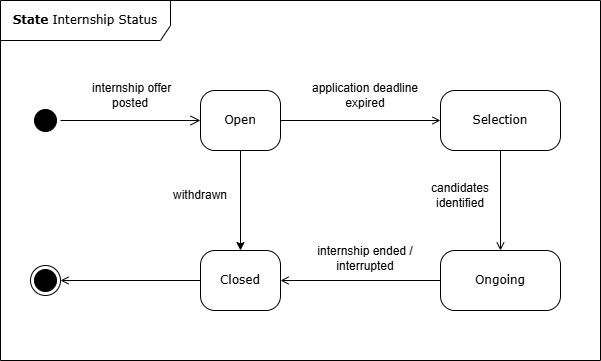
\includegraphics[width=1\linewidth]{LaTeXCode/images/State_diagram_internship.png}
        \caption{Internship Status State Diagram.}
        \label{fig:internship_state_diagram}%
    \end{center}
\end{figure}

This state diagram illustrates the lifecycle of an internship offer on the platform. It begins when an offer is posted, transitioning into the Open state, where the internship is available for applications. The offer remains open until either the application deadline expires, leading to the Selection phase, or the company withdraws it, moving directly to Closed. In the Selection state, candidates are evaluated, and if suitable candidates are identified, the process progresses to the Ongoing state, where the internship is actively taking place. Finally, upon completion or interruption of the internship, the offer transitions to the Closed state and it remains stored in the system.

\section{Product Functions}
\label{sec:product_functions}

The S\&C platform is designed to streamline the matching, selection and execution of internships, by providing functionalities that support every stage of the process. Key features include internship publication and search, automated recommendations, and monitoring tools. By integrating communication functionalities and feedback mechanisms, the platform ensures an effective experience for all users.

\begin{itemize}

    \item \textbf{Sign Up and Profile Creation} \\
    Users, identified as Students, Companies, and Universities, must sign up to the platform in order to access its functionalities. During the registration process, they create profiles by providing required personal and professional details. For students, details include additional information such as experiences, skills, and attitudes, enabling the platform to generate accurate recommendations.
    For companies, it also includes the fields in which they operate and eventually their branding elements.

    \item \textbf{Internship Publication} \\
    The platform enables companies to publish detailed and descriptive internship opportunities.
    Relevant information includes the application domain of the project along with the tasks that the student will be required to perform with the adopted technologies, if applicable.
    Furthermore, the details include the terms offered by companies: paid internship, training period or other benefits.
    These details are essential for allowing students to make informed decisions and to improve the recommendation algorithm. Companies are allowed to withdrawn internship offers before the application deadline expires.

    \item \textbf{Internship Search} \\
    Students can search for internship opportunities using filtering options based on standardized information required by the platform while posting an internship offer. This functionality ensures a user-friendly browsing experience, allowing students to efficiently find internships aligned with their preferences.

    \item \textbf{Generation of Recommendations} \\
    The platform automatically generates recommendations for students based on their profiles and, asymmetrically, suggests suitable candidates to companies. 
    The system employs various strategies to provide accurate and relevant suggestions.
    Both parties can evaluate the received recommendations and decide to accept or decline them based on their interests.

    \item \textbf{Support in the Selection Process} \\
    The platform facilitates the selection process by enabling companies to contact the candidates, schedule interviews and collect responses from students to questions shared by the company for their evaluation. In the end, it reports to students the outcomes of their interviews.

    \item \textbf{Communication Functionalities and Monitoring} \\
    The platform supports communication between students and companies, allowing them to provide updates about the status and progress of their ongoing internships and monitor them. 
    Communication of problems and complaints is made possible through private spaces.
    Universities can monitor internships to handle complaints and issue them when possible, interrupting internships if necessary.

    \item \textbf{Collecting Feedback} \\
    To improve its recommendation system, the platform gathers feedback from students and companies both during and after internships. This feedback loop allows a continuous refinement, to better address the interests of parties over time.

    \item \textbf{Personalized Suggestions} \\
    The platform assists users by providing personalized suggestions to produce more appealing descriptions. In particular, it provides suggestions to students for improving their profiles and
    it offers guidance to companies on how to optimize their internship descriptions.
\end{itemize}

\subsection{Requirements}
\label{subsec:requirements}

\newcounter{req}
\setcounter{req}{1}
\newcommand{\creq}{\thereq\stepcounter{req}}

In this section, the requirements for the system to be developed are outlined:

%Format: [condition][subject][action][object][constraint of action]
        
        \textbf{[R\creq]} Upon request, the system shall allow the User to sign up to the platform, as long as they submit all the required information, they don't already have a profile in the platform and their identity and role (Student, Company or University) are verified.

        \textbf{[R\creq]} Upon request, the system shall allow the requesting User to log in to the platform, granting him access to their profile as long as their authentication is successful.

        \textbf{[R\creq]} Upon request, the system shall allow the requesting User to update their profile, as long as they provide all the necessary information.

        \textbf{[R\creq]} Upon request, the system shall allow a Company to publish a new internship offer, as long as it provides all the required information and the latter is compliant with platform guidelines.

        \textbf{[R\creq]} Whenever a Company publishes an internship offer, the system shall add it to the list of all the internship offers.

        \textbf{[R\creq]} Upon request, the system shall allow the requesting Company to update information for any of their open internship offers, as long as it provides all the necessary information.

        \textbf{[R\creq]} Upon request, the system shall allow the requesting Company to withdraw any of their open internship offers.
        
        \textbf{[R\creq]} Upon request, the system shall allow a Student to search for desired internship offers by applying optional filters to the list.

        \textbf{[R\creq]} Whenever receiving a list of filter attributes for searching internship offers, the system shall return the list of all the offers matching the selected criteria.

        \textbf{[R\creq]} Upon request, the system shall allow the requesting Student to apply to an internship offer, as long as that offer's application deadline has not expired.

        \textbf{[R\creq]} Whenever a Student applies for an internship offer, the system shall add them to the list of candidates for that offer.

        \textbf{[R\creq]} Whenever a Student applies for an internship offer, the system shall mark all the "Unhandled" recommendations of that Student about that internship offer as "Accepted".

        \textbf{[R\creq]} Whenever a Student applies for an internship offer, the system shall discard all the "Unhandled" recommendations of the Company offering it about that Student in the context of that offer.

        \textbf{[R\creq]} Whenever an internship offer is withdrawn by its publishing Company, the system shall discard all applications to that offer.

        \textbf{[R\creq]} Whenever an internship offer is withdrawn by its publishing Company, the system shall discard all generated recommendations linked to that offer.

        \textbf{[R\creq]} Whenever a recommendation aimed at a Party is generated, the system shall add that recommendation to that Party's profile, as long as there is not another "Unhandled" recommendation about the other Party in the context of the same offer.

        \textbf{[R\creq]} Whenever a new Student signs up to the platform, the system shall generate, for every internship offer matching that Student's data, a recommendation about them aimed at the Company advertising that offer, as long as the latter's application deadline has not expired.

        \textbf{[R\creq]} Whenever a Student updates their profile, the system shall generate, for every internship offer matching that Student's updated data, a recommendation about them aimed at the Company advertising that offer, as long as the latter's application deadline has not expired.

        \textbf{[R\creq]} Whenever a Company publishes a new internship offer, the system shall generate, for every Student matching with that internship offer's data, a recommendation about it aimed at that Student.

        \textbf{[R\creq]} Whenever a Company updates data for an internship offer, the system shall generate, for every Student matching with that internship offer's updated data, a recommendation about it aimed at that Student.

        \textbf{[R\creq]} Whenever an internship offer is withdrawn by its publishing Company or its application deadline expires, the system shall discard all the recommendations about it, regardless of whether they have been accepted or not.

        \textbf{[R\creq]} Upon request, the system shall allow the requesting Party to manage their received recommendations by accepting or refusing them, if those have not already expired.

        \textbf{[R\creq]} Whenever a Student accepts one of their received recommendations, the system shall apply the requesting Student to the internship offer to which the recommendation refers.

        \textbf{[R\creq]} Whenever a Company accepts one of their received recommendations, the system shall generate a symmetric recommendation to the corresponding Student and add it to the latter's list of recommendations, as long as the generated recommendation is not already present in it.

        \textbf{[R\creq]} After the application deadline of an internship has expired, the system shall allow the publishing Company to contact a Student who had previously applied to that offer in order to plan a future interview with them, if none has been planned yet.

        \textbf{[R\creq]} Whenever a Student receives an interview proposal, the system shall allow that Student to either accept it or refuse it by providing a reason.

        \textbf{[R\creq]} Whenever an interview has to be carried out in-platform, the system shall allow the interviewing Company to submit questions to the Student involved.

        \textbf{[R\creq]} Whenever a Company submits questions to a Student for an in-platform interview, the system shall allow that Student to answer those questions, reporting them to the interviewing Company.

        \textbf{[R\creq]} Upon request, the system shall allow a Company to evaluate the answers received from a Student in one of their interviews, by registering that interview's result.

        \textbf{[R\creq]} Whenever a Company evaluates an interview (both in-platform and in-person), the system shall inform the corresponding Student of the registered outcome.  

        \textbf{[R\creq]} Whenever the interview results for all the candidates for an internship offer have been registered into the platform, the system shall close the selection process of that offer. 

        \textbf{[R\creq]} Upon request, the system shall allow the requesting Party to provide new information about any of the ongoing internships in which that Party is involved.

        \textbf{[R\creq]} Upon request, the system shall yield to the requesting Party all the information about one of the ongoing internships it is involved in.

        \textbf{[R\creq]} Upon request, the system shall allow the requesting Party to report a problem occurring in one of the ongoing internships it is involved in.

        \textbf{[R\creq]} When receiving a problem report about an internship from a Party, the system shall forward it to the University of the Student involved in that internship.

        \textbf{[R\creq]} Upon request, the system shall allow the requesting University to handle a received problem regarding an ongoing internship in which one of its Students is taking part.

        \textbf{[R\creq]} Upon request, the system shall allow the requesting Party to report feedback about an internship in which it has been actively involved, if that internship has been completed.

        \textbf{[R\creq]} Whenever receiving feedback about a completed internship, the system shall process it in order to improve the process for generating recommendations for the future.

        \textbf{[R\creq]} Upon request, the system shall provide a Student with targeted suggestions for optimizing its profile, enabling the Student to improve its appeal and relevance for obtaining more internship offers in the future, if such optimizations can be found.

        \textbf{[R\creq]} Upon request, the system shall provide a Company with targeted suggestions for optimizing a selected internship offer, enabling the Company to make it more attractive to Students and to improve its visibility for the future, if such optimizations can be found.
        
\section{User Characteristics}
\label{sec:User_characteristics}%

The S\&C platform is designed for three categories of users:

\begin{itemize}
    \item [\textbf{Students}] University students seeking internships. They are typically proficient users, familiar with app navigation and common interaction patterns such as registration, profile management, and document uploads (e.g., CVs). Their primary motivation is to find internships aligned with their skills and career goals efficiently. Students generally access the platform a few times each week while searching for internships and reviewing recommendations, with increased frequency during the interview phases.
    
    \item [\textbf{Companies}] Human Resources professionals responsible for posting internship opportunities, reviewing candidate recommendations, conducting the selection process, and providing feedback on ongoing internships. These users may vary in technical proficiency with the platform, but expect a straightforward interface to accomplish core tasks efficiently.
    They typically interact with the platform multiple times daily during work hours, particularly during active recruitment periods.
    
    \item [\textbf{Universities}] University staff responsible for monitoring internship outcomes and addressing their student-related complaints during internships. While their technical expertise may vary, they require tools for monitoring and complaint management. They have minimal involvement in day-to-day activities on the platform. The typical number of interactions can be a few times per week, depending on the number of students they manage.
\end{itemize}

All users expect a user-friendly interface, reliable notifications, and support features. The system accommodates varying levels of technical proficiency and ensures accessibility for all user groups.

\section{Assumptions, Dependencies and Constraints}
\label{sec:assumptions_dependencies_constraints}%

\subsection{Domain Assumptions}
\label{subsec:domain_assumptions}%

\newcounter{da}
\setcounter{da}{1}
\newcommand{\cda}{\theda\stepcounter{da}}

    \textbf{[DA\cda]} Users always interact with the system only through a device with a reliable connection to the Internet.

    \textbf{[DA\cda]} People who sign up to the platform have an active email address that they can provide to the system.

    \textbf{[DA\cda]} People who sign up to the platform can access the mailbox of the email address provided during the registration process.

    \textbf{[DA\cda]} People who are not Students, Companies or Universities never disguise themselves as being one of those.

    \textbf{[DA\cda]} Students signing up to the platform belong to one of the Universities which have already registered on the platform.

    \textbf{[DA\cda]} Users never provide false information about themselves.

    \textbf{[DA\cda]} Companies never provide false information about their internship offers.

    \textbf{[DA\cda]} Students never withdraw any of their applications to internship offers (equivalently, they apply for internships only if those match their interests and if they really want to undertake them).

    \textbf{[DA\cda]} For each of their internship offers, Companies always try to set up interviews with all and only the Students who have submitted an application.

    \textbf{[DA\cda]} Companies always finalize the selection process and bring it to completion, even if they haven't found any fitting candidate among the interviewed students.

    \textbf{[DA\cda]} Complaints inserted into the system always refer to events that have happened during the internship they are related to.

    \textbf{[DA\cda]} Users regularly upload information about the ongoing internships

    \textbf{[DA\cda]} Universities always act on received complaints and solve exposed issues, promptly terminating the internship if necessary.

    \textbf{[DA\cda]} Feedback inserted into the system after performing an internship is always meaningful to be fed to the statistical analysis.    

\begin{center}
\end{center}